\chapter{Results}%
\label{chap:results}
\textit{This chapter presents the test results that test and challenge the proposed framework.  The randomization tests, which additionally test the influence of the \ac{kgraph} and test taken including and excluding the \ac{kgraph}. The test results provide evidence that supports the effectiveness of the proposed framework. This chapter starts by introducing \textbf{method metrics} that indicate how a task has been executed by the proposed framework in \Cref{sec:proposed_method_metrics}. A comparison is made with the state-of-the-art methods in \Cref{sec:compare_with_related_papers}. \bs}

\paragraph{The Simulation Environment}
Testing in a simulation environment has been done using the URDF Gym Environment~\cite{spahn_urdfenvironment_2022}, a 100\% python environment build upon the PyBullet library~\cite{coumans_pybullet_2016}. The code created during the thesis can be found on \href{https://gitlab.tudelft.nl/airlab-delft/msc_projects/msc_gijs_groote}{GitLab} and \href{https://github.com/GijsGroote/semantic-thinking-robot}{GitHub}. Experiments ran on standard TU Delft laptop: HP ZBook Studio x360 G5, running OS:~Ubuntu 22.04.1 LTS x86\_64, CPU: Intel i7-8750H (12) @ 4.100GHz, GPU: NVIDIA Quadro P1000 Mobile.\bs
The simulation environment provides many different robots, of which two simple robots are selected to perform tests, they are displayed in \Cref{fig:example_robots}, and various objects are displayed in \Cref{fig:example_objects}.

\section{Proposed Method Metrics}%
\label{sec:proposed_method_metrics}

The results are measured in method metrics (\ac{pe}, search-, exeute- and total time to complete a task). The method metrics must not be confused with the monitoring metrics in \Cref{sec:monitoring_metrics} or the edge metrics in \Cref{subsec:edge_metrics}. The results are interesting, but most interesting is the progression of the method metrics over time. As will be shown, the effect of learning can be measured by investigating and tracking the method metrics over time. Furthermore, the method metrics will be used to compare the proposed framework to relative state-of-the-art papers. First, the method metrics are presented in~\Cref{table:proposed_method_metrics} with corresponding argumentation on the relevance of the metric.\bs

\noindent
\begin{table}[H]
\centering
\begin{tabular}%
  {>{\raggedright\arraybackslash}p{0.25\textwidth}%
   >{\raggedright\arraybackslash}p{0.65\textwidth}}
Total Average\newline \acl{PE} & The total average \ac{PE} is calculated by augmenting every prediction error into a single list, then the mean and standart deviation are calculated over that list. Since the \ac{PE} is high when unexpected behaviour occurs, seeing the total average \ac{PE} lower would indicate the robot encounters less unexpected behaviour, indicating the robot is learning.\\
% Total Average\newline \acl{TE}& The total average \ac{TE} is created by averaging over every hypothesis' average \ac{TE} in a \ac{hgraph}. Seeing the total average \ac{TE} lower over time would indicate the robot is selecting better suitable controllers and system models, indicating the robot is learning.\\
% Final positions and\newline displacement errors & The final position and displacement error is a metric which how a controller performs. This thesis does not create or investigate controllers, but it is interesting to see why different controllers are preferred for different objects. The final position and displacement error could be the cause.\\
% The ratio between the number of hypotheses and the number of tasks & Expected is that whilst learning system models, the hypothesis created will be more effective. Thus the ratio between the total number of hypotheses and the total number of tasks is expected to lower with new knowledge.\\
% The ratio between the number of successful and the number of total edges in \ac{kgraph} & When the \ac{kgraph} improves recommending a controller and system model, the ratio between successful edges and total edges is expected to increase because, with better recommendations, more edges will be completed.\\
task completion time =\newline run time + planning time& If equal tasks are given multiple times, the total task completion time should drop pretty drastically. Multiple factors help to lower the task completion time, firstly system identification has to be performed only once, and there is no need to lose time on redoing system identification. Secondly, the \ac{hgraph} is expected to improve generated hypothesis, or better said, the same mistake should not be made multiple times, resulting in fewer failing hypotheses and lowering task completion time.\\
\end{tabular}
\caption{Proposed method metrics used to compare the proposed framework with the state-of-the-art.}\label{table:proposed_method_metrics}
\end{table}


The  point robot is used during tests, the robot takes an velocity input along the \gls{x}- and in \gls{y}-axis, defined as:\bs

\[ u(k) = {[ u_{\gls{x}}(k), u_{\gls{y}}(k) ]}^\top \]

For tests, three system models are used, a \ac{LTI} model describing robot driving, and two nonlinear model describing the robot pushing an object. First a short textual description of the available system models is provided below. Second, the state space model is provided for the three implemented models.\bs

\noindent
\begin{table}[H]
\centering
\begin{tabular}%
  {>{\raggedright\arraybackslash}p{0.25\textwidth}%
   >{\raggedright\arraybackslash}p{0.65\textwidth}}
\textit{lti-drive-model} & A second order \ac{LTI} model that can be used by both the \ac{MPC} and the \ac{MPPI} drive controller. The next robot configuration is based on the current configuration and system input in \gls{x} and \gls{y} direction. \\
\textit{nonlinear-push-model-1} & A nonlinear model describing the next object configuration in \gls{x} and \gls{y} direction and the orientation \gls{theta} based on the current configurations of the robot, the object and on the robot inputs in \gls{x} and \gls{y} direction.\\
\textit{nonlinear-push-model-2} & A nonlinear model describing the next object configuration in \gls{x} and \gls{y}, and the object configuration in \gls{x} and \gls{y} direction based on the current configurations of the robot, the object and on the robot inputs in \gls{x} and \gls{y} direction.\\
\end{tabular}
\caption{Available drive and push system models.}\label{table:available_system_models}
\end{table}

State space representation of the \textit{lti-drive-model}:\bs

\begin{equation}
\label{eq:lti-drive-model}
x_{\mathit{lti-drive-model}}(k+1)=
\begin{bmatrix}
\gls{x}_\mathit{robot}(k+1)\\
\gls{y}_\mathit{robot}(k+1)
\end{bmatrix}
=
\begin{bmatrix}
\gls{x}_{\mathit{robot}}(k) + \gls{DT} u_{\gls{x}}(k)\\
\gls{y}_{\mathit{robot}}(k) + \gls{DT} u_{\gls{y}}(k)
\end{bmatrix}
\end{equation}

State space representation of the \textit{nonlinear-push-model-1}:\bs

\begin{equation}
x_{\mathit{nonlinear-push-model-1}}(k+1)=
\begin{bmatrix}
\gls{x}_{\mathit{robot}}(k+1)\\
\gls{y}_{\mathit{robot}}(k+1)\\
\gls{x}_{\mathit{obj}}(k+1)\\
\gls{y}_{\mathit{obj}}(k+1)
\end{bmatrix}
=
\begin{bmatrix}
\gls{x}_{\mathit{robot}}(k+1) + \gls{DT} u_{\gls{x}}(k)\\
\gls{y}_{\mathit{robot}}(k+1) + \gls{DT} u_{\gls{y}}(k)\\
\gls{x}_{\mathit{obj}}(k+1) + \frac{1}{2} \gls{DT} u_{\gls{x}}(k)\\
\gls{y}_{\mathit{obj}}(k+1) + \frac{1}{2} \gls{DT} u_{\gls{y}}(k)
\end{bmatrix}
\label{eq:nonlinear-push-model-1}
\end{equation}


State space representation of the \textit{nonlinear-push-model-2}:\bs
\begin{equation}
x_{\mathit{nonlinear-push-model-2}}(k+1)=
\begin{bmatrix}
\gls{x}_{\mathit{robot}}(k+1)\\
\gls{y}_{\mathit{robot}}(k+1)\\
\gls{x}_{\mathit{obj}}(k+1)\\
\gls{y}_{\mathit{obj}}(k+1)\\
\gls{theta}_{\mathit{obj}}(k+1)
\end{bmatrix}
=
\begin{bmatrix}
\gls{x}_{\mathit{robot}}(k) + \gls{DT} u_{\gls{x}}(k)\\
\gls{y}_{\mathit{robot}}(k) + \gls{DT} u_{\gls{y}}(k)\\
\gls{x}_{\mathit{obj}}(k) + \gls{DT}\sin(\gls{theta}_{\mathit{obj}}(k)) (1-|\frac{2\mathit{st}}{H}|)\mathit{vp}\\
\gls{y}_{\mathit{obj}}(k) + \gls{DT}\cos(\gls{theta}_{\mathit{obj}}(k)) (1-|\frac{2\mathit{st}}{H}|)\mathit{vp}\\
\gls{theta}_{\mathit{obj}}(k) + \frac{2*\gls{DT}*\mathit{vp}*\mathit{st}}{H}
\end{bmatrix}
\label{eq:nonlinear-push-model-2}
\end{equation}

Where \textit{st} indictates the distance from the contact point between the robot and pushed object, perpendicular to the line that coinsides with the object and the robots center of mass. A positive \textit{st} indicates the object will rotate anticlockwise, a negative \textit{st} indicates a clockwise rotation. The width of an object is defined as \textit{H}and is set to 2 meter, \textit{vp} is the velocity of the robot perpendicular to the objectdefined as

\[ \mathit{vp} = u_{\gls{x}} \sin(\gls{theta}_{\mathit{obj}}(k)) + u_{\gls{y}}\cos(\gls{theta}_{\mathit{obj}}(k)) \]

The goal of this thesis is not to find optimal control, or to model the environment with astonishing accurately. The goal is to select the best combination of controller and system model in the available set of controllers and system models.

% \begin{figure}[H]
%     \centering
%     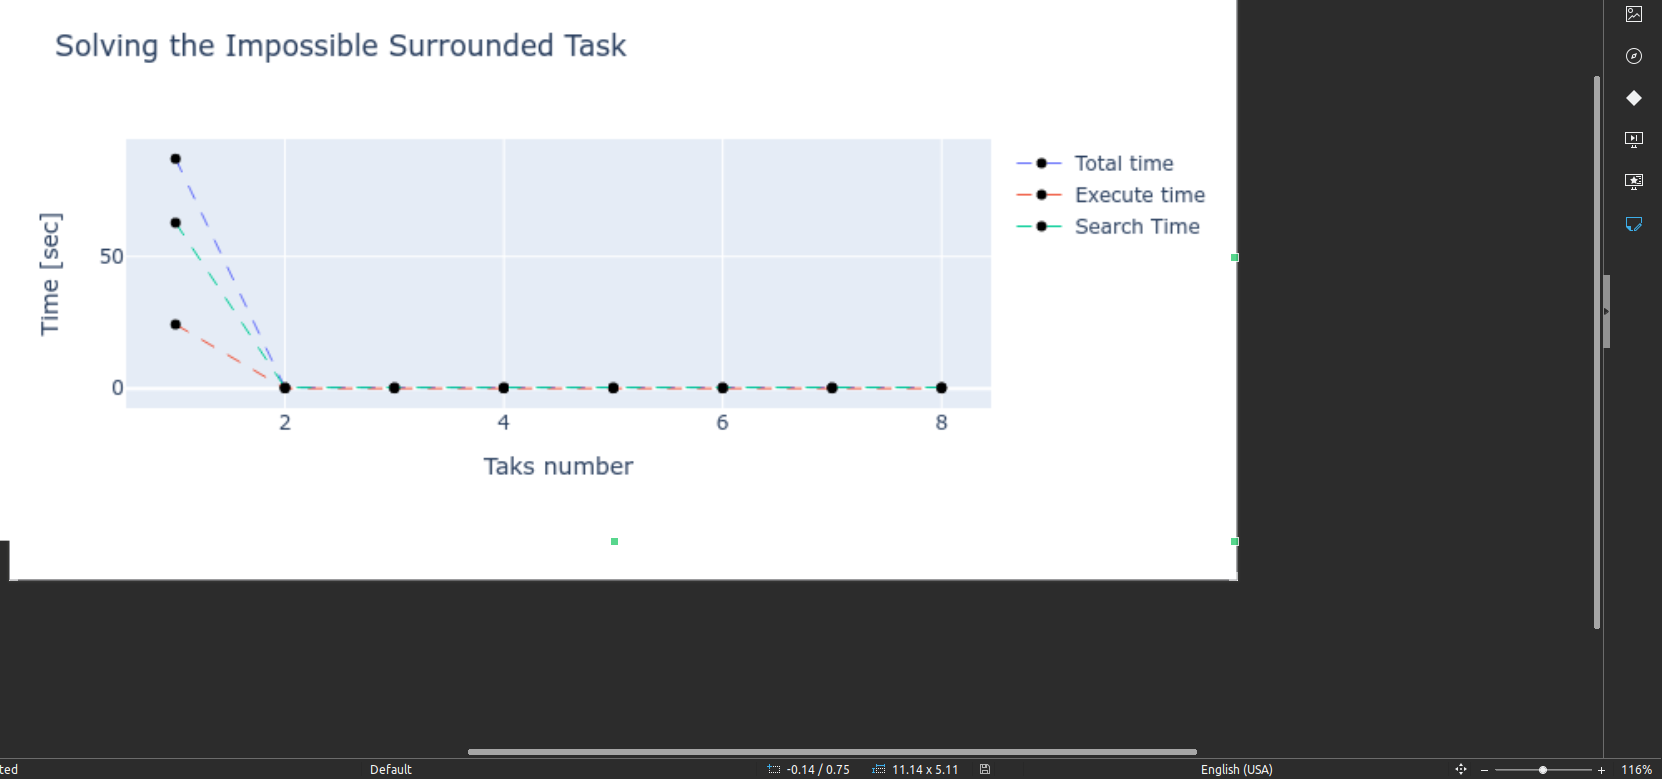
\includegraphics[width=5cm]{figures/results/execution_time_move_2}
% figures/figures/figures/figures/
%     \caption{}%
%     \label{}
% \end{figure}


% \section{Benchmark Tests}%
% \label{sec:benchmark_tests}
% Three benchmark test are presented, starting with the blockade task. A large part of the proposed framework is system identification, for testing however no system identification is performed. Instead, several hard-coded system models are used, and the \ac{kgraph} finds which system model is the best choice for an object over time. Where the best choice is defined using the edge metrics discussed in \Cref{subsec:edge_metrics}. The hard-coded system models are not opting for modelling the drive or push model as accurately as they possibly can, thus severe model mismatch should be expected. Such model mismatch is no issue, to complete a subtask stable closed-loop control is required, when an edge parameterization is unable to provide closed-loop stable control, the edge will fail because a fault will be detected. To answer the research question, improvement over time should be made. Gaining such improvement does not require accurate system models, time spend improving the hand-coded system models does thus not change the result.\bs
%
%
% \paragraph{Blockade} In the blockade environment the robot is tasked with placing a box in a target position that is blocked by a cylinder object.\bs
% \begin{figure}[H]
%     \centering
%     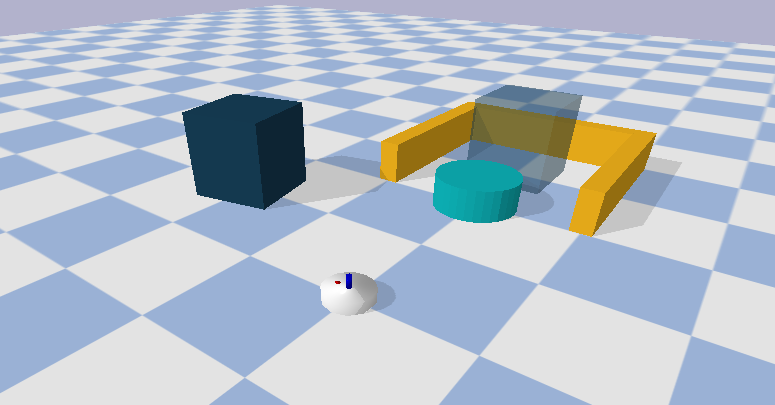
\includegraphics[width=0.9\textwidth]{figures/results/blockade}
%     \caption{The blockade environment with the target ghost position for the blue box. The green walls are unmovable whilst both the blue box and cylinder are movable.}%
%     \label{fig:benchmark_blockade}
% \end{figure}
%
% The blockade task neatly shows that the \ac{halgorithm} uses the backward search technique. First, the \ac{halgorithm} plans to push the box directly to the target position, then it realizes a blocking object must first be moved to free the path. It makes the mistake of pushing the unmovable wall, then it succeeds in pushing the movable cylinder out of the way. The \ac{kgraph} then ensures that this mistake will not occur again because is remembered that the wall is immovable. Over time the \ac{kgraph} indicates that it prefers to use the \ac{MPPI} controller with the nonlinear-push-model-2 to push both the box and the cylinder object. Converging to this conclusion improves the method metrics for the task as can be seen in \Cref{fig:results_blockade}\bs
%
% \todo[inline]{is nonlinear-push-model-2 still the preferred model after testing??}
%
% \begin{figure}[H]
%     \centering
%     
\includegraphics[width=0.9\textwidth]{figures/tests/404_not_found}
%
%     \caption{Some results are still under development for the blockade environment}%
%     \label{fig:results_blockade}
% \end{figure}
% \todo[inline]{Test to create results for running the blockade environment, and input into above 404 not found}
%
% \paragraph{Swap}
% In the swap environment the robot should swap the locations of the 2 objects in the environment.\bs
%
% \begin{figure}[H]
%     \centering
%     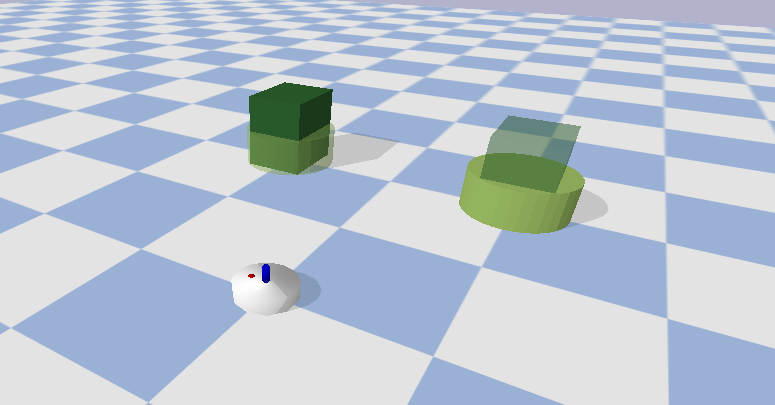
\includegraphics[width=0.9\textwidth]{figures/results/swap}
%     \caption{The swap environment, the robot is tasked with swapping the positions of the cylinder and the box.}%
%     \label{fig:benchmark_swap}
% \end{figure}
% The swap task shows that the \ac{halgorithm} can handle overlapping subtasks. The \ac{halgorithm} handles a single subtask at a time and randomly selects which subtask to handle next. The result for the swap task is that first, the robot will place the box on the location of the cylinder. The cylinder is blocking the path and is thus pushed to free the path, then the robot drives back to the box to push the box to its target position. The cylinder can directly be pushed toward its target position, because there is a free path, and the task is successfully completed. By manual inspection, this is the most efficient action sequence to complete the swap task. But there is an assumption because the initial environment has a distance between the robot and box (robot-box distance), and robot and cylinder (robot-cylinder distance) that is equal. If the initial robot-box distance is greater than the initial robot-cylinder distance, it would be more efficient to first drive toward the cylinder because that distance is smaller. The selection of subtask is random, thus there is a 50\% chance that the robot selects a subtask resulting in driving more than is necessary to complete the swap subtask.\bs
%
% \begin{figure}[H]
%     \centering
%     
\includegraphics[width=0.9\textwidth]{figures/results/404_not_found}
%     \caption{Some tests are still under development for the swap environment}%
%     \label{fig:results_swap}
% \end{figure}
%
% \todo[inline]{Test to create results for running the swap environment}
%
% \paragraph{Surrounded} In the surround environment the robot has to learn which box is movable to escape the enclosure of boxes.\bs
% \begin{figure}[H]
%     \centering
%     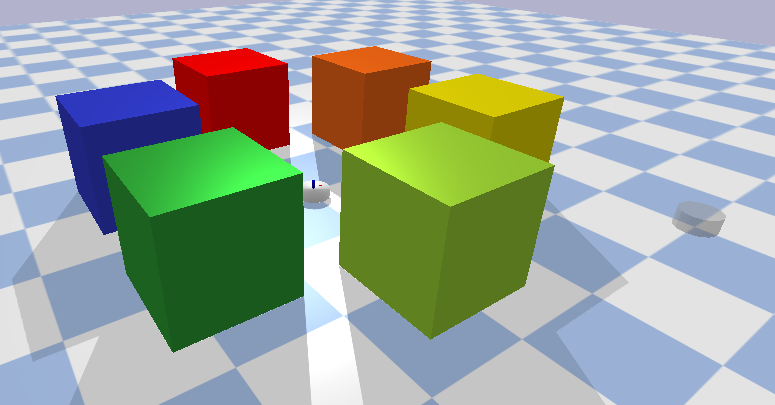
\includegraphics[width=0.9\textwidth]{figures/results/surrounded}
%     \caption{The surround environment, the robot is tasked with escaping the surrounding enclosure by driving to the target ghost position displayed on the right side in the figure. Every box objects is unmovable except the red box which is movable.}%
%     \label{fig:benchmark_surround}
% \end{figure}
% The surround task show that having and gaining environment knowledge can greatly improve task execution. Simply knowing if an object can be interacted with may lower task execution time drastically as can be seen in \Cref{fig:results_surround}.\bs
%
% \begin{figure}[H]
%     \centering
%     
\includegraphics[width=0.9\textwidth]{figures/results/404_not_found}
%     \caption{Some test are still under development for the surround environment}%
%     \label{fig:results_surround}
% \end{figure}
%
% \todo[inline]{Test to create results for running the surround environment}

\section{Randomization}%
\label{sec:randomization}
In the randomized environment the task and the environment are initialised by randomization, after tasks completion, the environment is reshuffled. A reshuffled gives the objects in environment and task a new initial pose and resets the robot position. By solving a task, reshuffeling the environment and solving another reshuffled task, the robot gains experience that is stored in the \ac{kgraph}. A set of multiple tasks where initially the \ac{kgraph} is named a \textit{run}, and at the end of a run the \ac{kgraph} is filled with the gained experience. \Cref{table:configure_rand_env} presents a set of parameters that initializes the random environment. Two type of tasks solved by the robot, an driving task, where the robot must drive toward multiple random target poses, and a pushing task, where the robot must push an movable object toward a random target pose. First the of search- and execution time of a task is investigated, and its development when the robot gains more experience. Then a comparison is made between solving and reshuffling multiple tasks once with the \ac{kgraph} that suggests edge parameterisations, and once without suggestions and by random sampling over the availabel edge parameterizations.\bs

\noindent
\begin{table}[H]
\centering
\begin{tabular}%
{>{\raggedright\arraybackslash}p{0.25\textwidth}%
>{\raggedright\arraybackslash}p{0.65\textwidth}}
The \textit{size of the grid} & length and width of the ground plane in \gls{x} and \gls{y} direction.\\
The \textit{minimal and maximal size of objects} & A box will have sides with a length that lie in the specified range from minimal to maximal length. Cylinders will have a diameter and height that is within the specified range, additionally, cylinders are not higher than the radius of the cylinder to prevent cylinders from tipping over. \\
The \textit{maximal weight} & which is uniformly distributed for the environment objects, minimal weight is set by default to 1 gram. \\
The \textit{number of unmovable objects} & Specify the amount of unmovable objects.\\
The \textit{number of movable objects} & Specify the amount of movable objects.\\
The \textit{number of subtasks in a task} & Specify the amount of subtasks in a task.
\end{tabular}
\caption{The tuning parameters that must be specified for the random environment}%
\label{table:configure_rand_env}
\end{table}

The ratio between the number of cylinders and boxes is determined by randomization. For every new object generated there is a 50\% chance it becomes a box and 50\% chance it becomes a cylinder.

The environment can be \textit{reshuffled}, and can be visualise in \Cref{fig:random_environment_reshuffle}. Reshuffling the environment changes 3 aspects of the environment, first, the robots position is reset to the origin \gls{origin}. Second, every object is set to a new initial position whilst their properties are unchanged. Thirth and last, objects in the task receive new target poses.  The reshuffle functionality can be visualised in \Cref{fig:random_environment_reshuffle}. By solving a similar task in an reshuffled random environment multiple times, the robot gains experience and task exection can be investigated. With the investigation trends in task execution is monitored, to see improvement whilst gaining experience.\bs


\begin{figure}[H]
    \centering
    \begin{subfigure}{.49\textwidth}
    \centering
    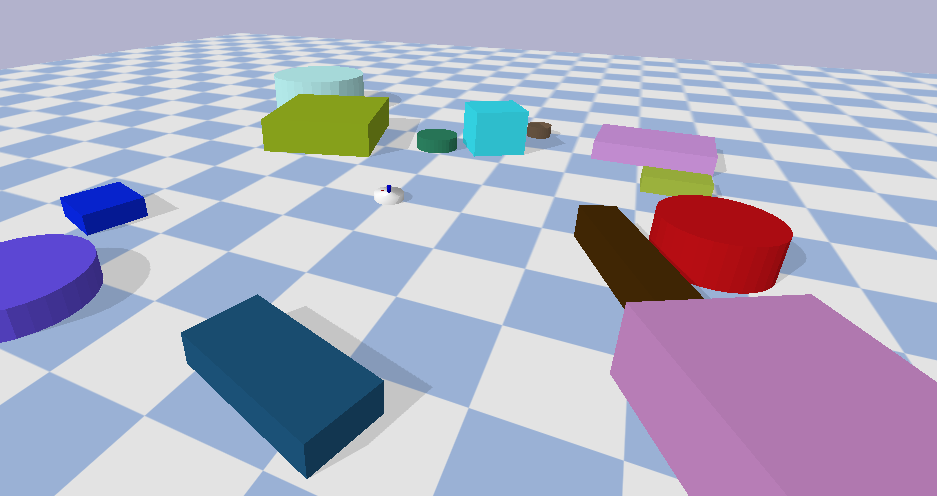
\includegraphics[width=\textwidth]{figures/results/random1}
    \end{subfigure}
    \hfill
    \begin{subfigure}{.49\textwidth}
    \centering
    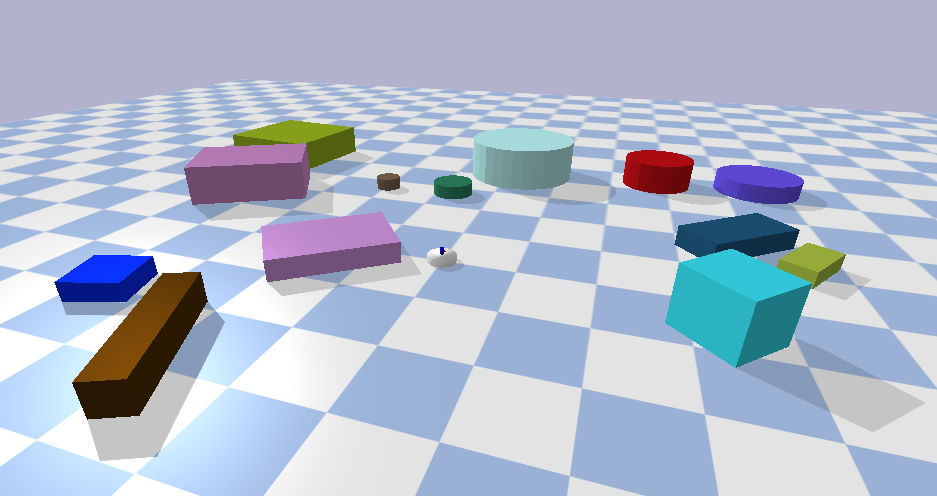
\includegraphics[width=\textwidth]{figures/results/random2}
    \end{subfigure}

    \vspace{0.2cm}
    \begin{subfigure}{.49\textwidth}
    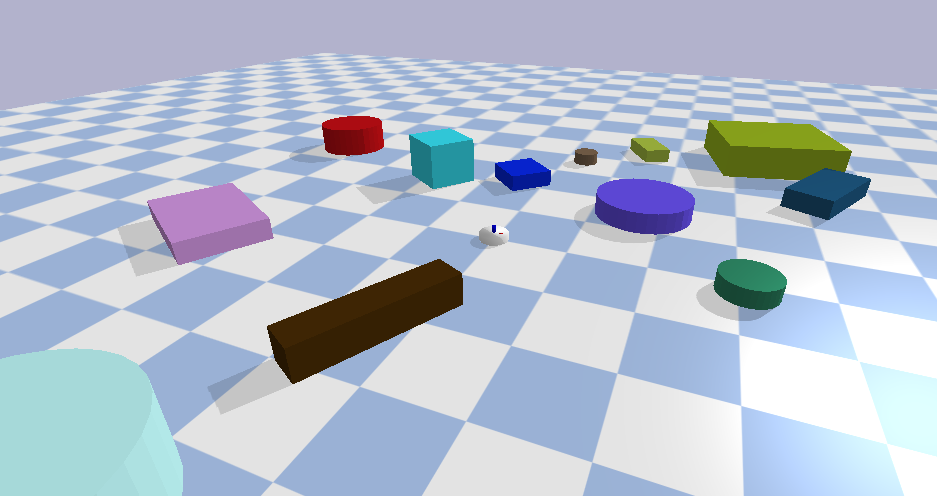
\includegraphics[width=\textwidth]{figures/results/random3}
    \end{subfigure}
    \hfill
    \begin{subfigure}{.49\textwidth}
    \centering
    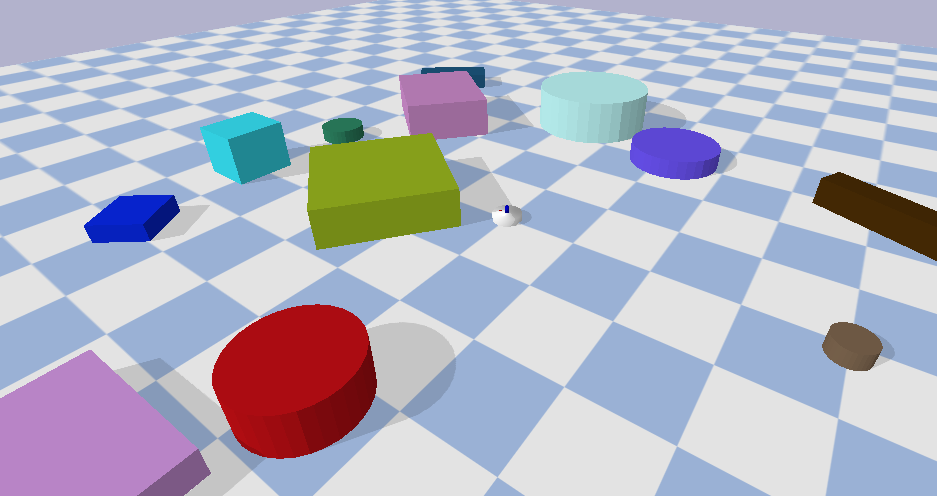
\includegraphics[width=\textwidth]{figures/results/random4}
    \end{subfigure}
    \caption{A random environment initialised by tuning parameters presented in \Cref{table:configure_rand_drive_env_values}. After initialisation the environment objects initial poses are reshuffled three times.}%
    \label{fig:random_environment_reshuffle}
\end{figure}

\subsection{A Driving Task}%
\label{subsec:rand_driving}
For the driving task the random environment is created with the following tuning parameters.\bs

\begin{table}[H]
\centering
\begin{tabular}%
{>{\raggedright\arraybackslash}p{0.30\textwidth}%
>{\raggedright\arraybackslash}p{0.60\textwidth}}
\text{grid size}  &\gls{x}=12 m, \quad \gls{y}=12 m \\
\text{object size}  &$\mathit{min\_length}=0.2 m, \quad \mathit{max\_length}=2 m$ \\
\text{object weight}  &$\mathit{max\_weight}=1000 g = 1 \mathit{kg}$\\
\text{number of objects}  &$\mathit{num\_unmovable\_obj}=3, \quad \mathit{num\_movable\_obj}=5$ \\
\text{number of tested runs}  &$\mathit{num\_runs}=10$\\
\text{number of tasks in a run}  &$\mathit{num\_tasks}=10$\\
\text{number of subtasks in a task}  &$\mathit{num\_subtasks}=3$
\end{tabular}
\caption{The selected tuning parameters for the randomised drive environment.}%
\label{table:configure_rand_drive_env_values}
\end{table}

These parameters have been specifically selected, starting with the size of the ground floor. The ground floor should be large enough such that objects can be pushed around, note that, for a driving task, pushing is involved when a path must be freed. An enormous (100 by 100 meter) ground floor would result in a longer computational time for path planning, which is undesired. A 12 by 12 meter ground floor is selected because the floor is large enough for objects to be pushed around. The range that determines the size of objects is set such that objects can be as large as the robot itself, and be around 10 times as large as the robot. With these sizes the robot is unable to grasp objects, a gripper would be too small to grasp objects. The comparatively large size fits the objective of nonprehensile pushing, there simply is no other method to manipulate such large objects other than pushing. A real-life example are can be found in harbours where tug boats push giant cargo ships around that are many times over the size of the tug boat. The ratio of solid obstacles vs.~movable objects determines if a task is more navigation (only solid obstacles) or more \ac{NAMO} (only movable objects). A task that tends toward \ac{NAMO} is favoured because that is the target environment in this thesis. There should be some unmovable obstacles that reward the robot learning such objects are unmovable (to then not interact with them). Thus there are more movable objects than solid obstacles chosen, whilst still having 2 solid obstacles around. Ten runs are taken, each run consisting of 10 tasks, the results are averaged to reach statistic relevance in a randomised environments. The number of subtasks is set to 3, a low number of drive subtasks that can be completed in under 2 minutes.\bs

Lastly, a number of tuning parameters must be set for the \ac{halgorithm}. These are the maximal robot speed, set to 1 $m/s$, the \textit{cell size} for the path estimator set to 0.1 meter, the action planner takes four tuning paramters; the \textit{step size} set to 0.2 meter, the \textit{search size} set to 0.35 meter, an \textit{known obstacle space cost} set to 2 meter and an \textit{unknown obstacle space cost} set to 3.5 meter.\bs

All parameters are set, results can be analysed, the following two figures show the execution-, search- and total times over the ten runs. First, a boxplot displaying task execution whilst using \ac{kgraph} action suggestions in \Cref{fig:random_drive_time_kgraph}, second, a boxplot displays task execution withouth using \ac{kgraph} action suggestions in \Cref{fig:random_drive_time_no_kgraph}.\bs

\begin{figure}[H]
    \centering
    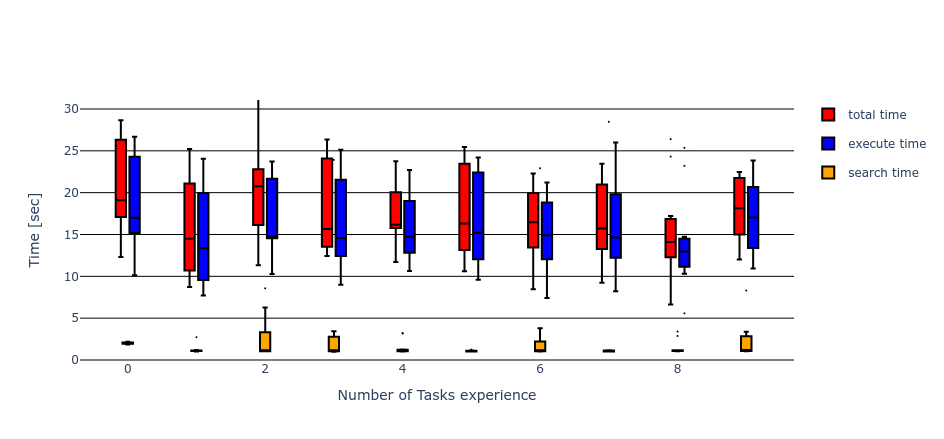
\includegraphics[width=\textwidth]{figures/results/random_drive_time_kgraph}
    \caption{Search-, execution- and total time to complete a drive task \textbf{whilst} using \ac{kgraph} action suggestions. The horizontal axis indicates the number of task experience in a run. A run contains ten tasks, starting the run with an empty \ac{kgraph} that collects action feedback as the robot gains experience. The task contains three subtasks, in other words, the robot must drive to three target poses in order to complete a task. The vertical axis displays a boxplot of the search-, execution- and total time over ten runs, where the sum of seach- and execution time equals total time.}%
   \label{fig:random_drive_time_kgraph}
\end{figure}

The above figure displays results where the \ac{halgorithm} sends action feedback and received action suggestions from the \ac{kgraph}, the figure below displays the results for solving the same tasks in the same random environment without using \ac{kgraph} suggestions. Instead a random parameterization is selected for every action edge. Ensuring that the random environments are repeatible is accomplished by fixing the seed. The fixed seed ensures that the randomly generated environments can be created multiple times, once to solve with \ac{kgraph} suggestions and once to solve without help from the \ac{kgraph}.\bs

\begin{figure}[H]
    \centering
    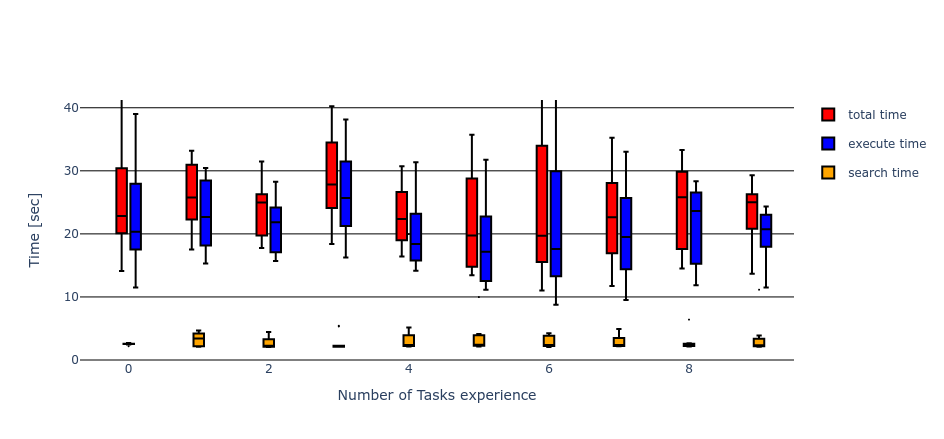
\includegraphics[width=\textwidth]{figures/results/random_drive_time_no_kgraph}
    \caption{Search-, execution- and total time to complete a drive task \textbf{withouth} using \ac{kgraph} action suggestions. The horizontal axis indicates the number of task experience in a run. A run contains ten tasks, starting the run with an empty \ac{kgraph} that collects action feedback as the robot gains experience. The task contains three subtasks, in other words, the robot must drive to three target poses in order to complete a task. The vertical axis displays a boxplot of the search-, execution- and total time over ten runs, where the sum of seach- and execution time equals total time.}%
   \label{fig:random_drive_time_no_kgraph}
\end{figure}


The results in both \Cref{fig:random_drive_time_kgraph,fig:random_drive_time_no_kgraph} show no clear trend. However overall \Cref{fig:random_drive_time_kgraph} shows significat improvement over \Cref{fig:random_drive_time_no_kgraph} which becomes better visable if only the means are compared in \Cref{fig:random_drive_time_vs}.\bs

\begin{figure}[H]
    \centering
    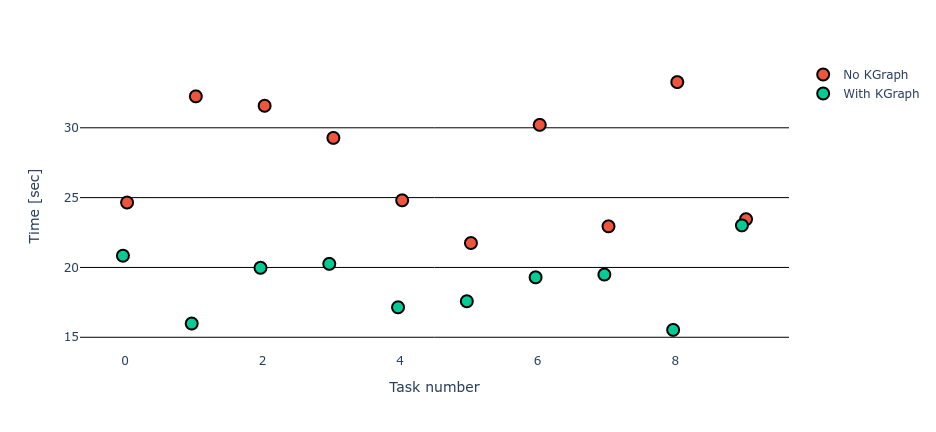
\includegraphics[width=\textwidth]{figures/results/random_drive_time_vs}
    \caption{Comparing average total time to complete a task out of then runs for a driving task. For the edge parameterizations once with the use of \ac{kgraph} action suggestions is leveraged indicated by \quotes{with \ac{kgraph}} and once with random selection indicted by \quotes{no \ac{kgraph}}.}%
    \label{fig:random_drive_time_vs}
\end{figure}

Two driving edge parameterisations are available, the \ac{MPC} and the \ac{MPPI} parameterisation that both use lti-drive-model. The \ac{kgraph} prefers the \ac{MPC} parameterization over de \ac{MPPI} parameterization as can be seen in \Cref{table:rand_drive_mpc_vs_mppi}. In this table is can be seen that the \ac{kgraph} needs at most one task of experience to suggest the \ac{MPC} parameterization. An explanation why there was no trend to be found in \Cref{fig:random_drive_time_kgraph}, it was alraedy converged at the first task.  

\begin{table}[H]
    \centering
    \begin{tabular}%
      {%
        >{\raggedright\arraybackslash}p{0.10\textwidth}
        >{\raggedright\arraybackslash}p{0.22\textwidth}
      |p{0.4cm}p{0.4cm}p{0.4cm}p{0.4cm}p{0.4cm}p{0.4cm}p{0.4cm}p{0.4cm}p{0.4cm}p{0.4cm}}
      \multicolumn{2}{c|}{Number of Tasks in experience} &0&1&2&3&4&5&6&7&8&9\\\toprule
      \multirow{4}{0.1\textwidth}{With \ac{kgraph} suggestions} 
      &Number of \ac{MPC} parameterizations&22&33&34&33&33&33&33&34&33&32\\
      &Number of \ac{MPPI} parameterizations&11&0&0&0&0&0&0&0&0&0\\
      & \ac{MPC} selected in total drive actions [\%]&67&100&100&100&100&100&100&100&100&100\\
      & \ac{MPPI} selected in total drive actions [\%]&33&0&0&0&0&0&0&0&0&0\\\midrule
      \multirow{4}{0.1\textwidth}{Without \ac{kgraph} suggestions} 
      &Number of \ac{MPC} parameterizations &14&14&12&12&17&16&17&19&16&11\\
      &Number of \ac{MPPI} parameterizations &19&19&21&21&17&17&18&14&17&22\\
      & \ac{MPC} selected from total drive actions [\%] &42&42&36&36&50&48&49&58&48&33\\
      & \ac{MPPI} selected from total drive actions [\%]&58&58&64&64&50&52&51&42&52&67\\
    \end{tabular}
    \caption{Selecting the (\ac{MPC}, \textit{lti-drive-model}) parameterization versus selecting the (\ac{MPPI}, \textit{lti-drive-model} parameterization for drive actions.}%
    \label{table:rand_drive_mpc_vs_mppi}
\end{table}

The \ac{halgorithm} succesfully completes 300 subtasks (3 subtasks per task, 10 tasks per run, 10 runs are compeleted) twice. Once while stroing edge feedback in the \ac{kgraph} that suggest edge parameterization, and once without \ac{kgraph}. In \Cref{table:rand_drive_mpc_vs_mppi} the number of \ac{MPC} and \ac{MPPI} parameterizations should be more than 30 for any number of tasks in experience. In many cases it is more than 30, which indicates more than 30 drive edges were created to complete 30 drive subtasks. A fault has been detected that terminates the execution of an edge, to complete the task, a new edge is created, resulting in more than 30 \ac{MPC} and \ac{MPPI} edge parameterizations. When comparing both a positive effect is measured of the use of the \ac{kgraph} on the total task required to complete a task compared to random selection of edge parameterization. Now a task is taken that compares the use of the \ac{halgorithm} with and without \ac{kgraph} for a pushing task.\bs

\subsection{A Pushing Task}%
\label{subsec:rand_pushing}
The push task in the randomized environment consists of a single subtask. To complete this push task the robot must push the an object toward its specified target pose. The tuning parameters that make up the random environment for the push task can be visualised in \Cref{table:configure_rand_push_env_values}.\bs

\begin{table}[H]
\centering
\begin{tabular}%
{>{\raggedright\arraybackslash}p{0.30\textwidth}%
>{\raggedright\arraybackslash}p{0.60\textwidth}}
\text{grid size}  &\gls{x}=12 m, \quad \gls{y}=12 m \\
\text{object size}  &$\mathit{min\_length}=0.2 m, \quad \mathit{max\_length}=2 m$ \\
\text{object weight}  &$\mathit{max\_weight}=1000 g = 1 \mathit{kg}$\\
\text{number of objects}  &$\mathit{num\_unmovable\_obj}=3, \quad \mathit{num\_movable\_obj}=5$ \\
\text{number of tested runs}  &$\mathit{num\_runs}=10$\\
\text{number of tasks in a run}  &$\mathit{num\_tasks}=6$\\
\text{number of subtasks in a task}  &$\mathit{num\_subtasks}=1$
\end{tabular}
\caption{The selected tuning parameters for the randomised push environment.}%
\label{table:configure_rand_push_env_values}
\end{table}




\begin{figure}[H]
    \centering
    \begin{subfigure}{\textwidth}
    \centering
    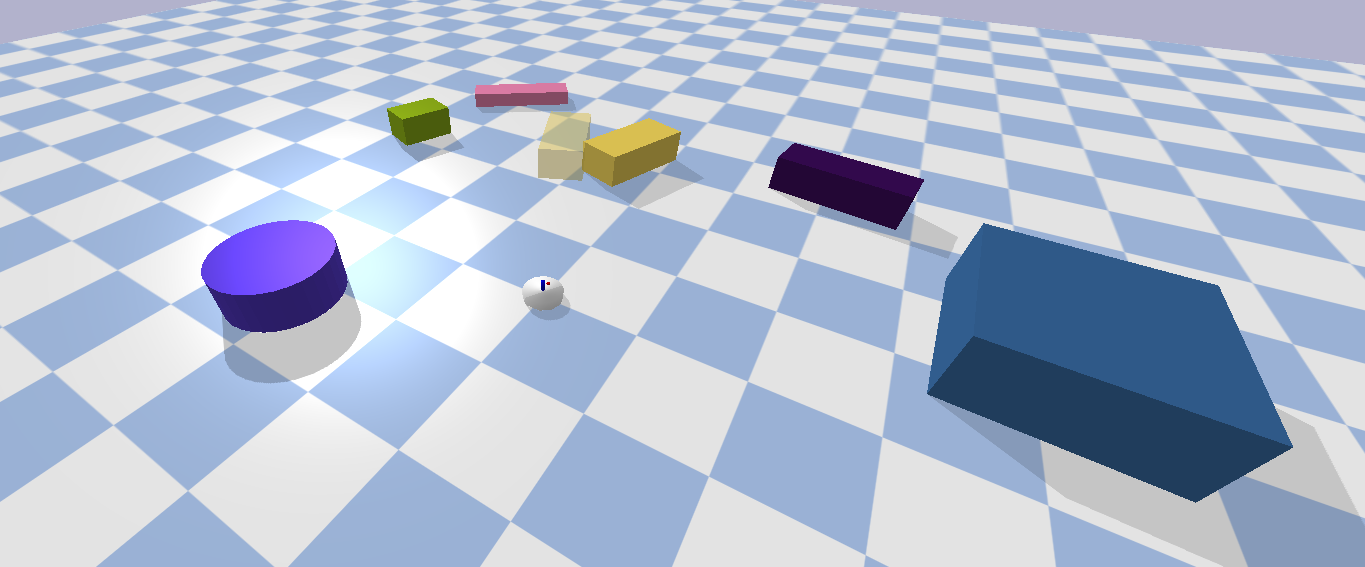
\includegraphics[width=0.9\textwidth]{figures/results/random_1}
    \end{subfigure}

    \vspace{0.2cm}
    \begin{subfigure}{\textwidth}
    \centering
    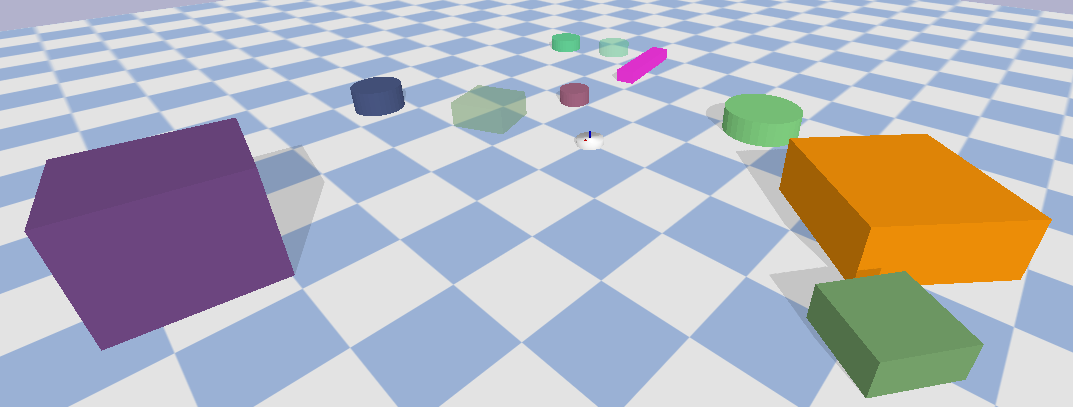
\includegraphics[width=0.9\textwidth]{figures/results/random_2}
    \end{subfigure}
    \caption{Two random environments where the task contains a subtask displayed by a target ghost pose.}%
    \label{fig:random_environnment}
\end{figure}

All tuning parameters are set up, now the results are presented, first the pushing task is completed using \ac{kgraph} suggestions. The search-, execute- and totaltime for task completion is presented in \Cref{fig:random_push_time_kgraph}. Then the same tasks are completed without help of the \ac{kgraph} suggestions in \Cref{fig:random_drive_time_no_kgraph}. 

\begin{figure}[H]
    \centering
    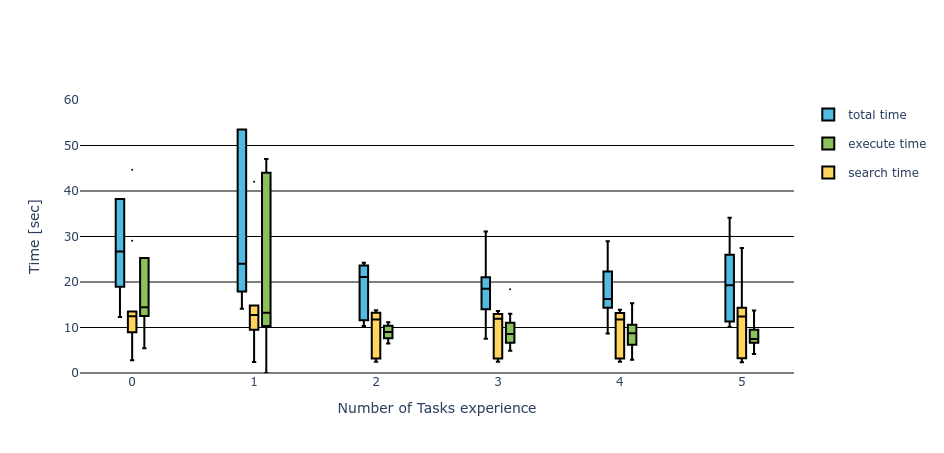
\includegraphics[width=\textwidth]{figures/results/random_push_time_kgraph}
    \caption{Search-, execution- and total time to complete a pushing task \textbf{with} \ac{kgraph} action suggestions. The horizontal axis indicates the number of task experience in a run. A run contains ten tasks, starting the run with an empty \ac{kgraph} that collects action feedback as the robot gains experience. The vertical axis displays a boxplot of the search-, execution- and total time over ten runs, where the sum of seach- and execution time equals total time.}%
    \label{fig:random_push_time_kgraph}
\end{figure}

\begin{figure}[H]
    \centering
    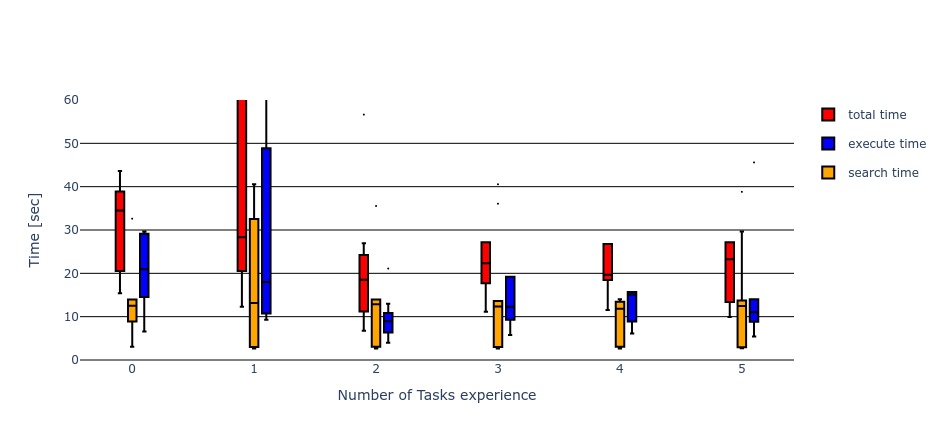
\includegraphics[width=\textwidth]{figures/results/random_push_time_no_kgraph}
    \caption{Search-, execution- and total time to complete a pushing task \textbf{without} \ac{kgraph} action suggestions. The horizontal axis indicates the number of task experience in a run. A run contains ten tasks, starting the run with an empty \ac{kgraph} that collects action feedback as the robot gains experience. The vertical axis displays a boxplot of the search-, execution- and total time over ten runs, where the sum of seach- and execution time equals total time.}%
    \label{fig:random_push_time_no_kgraph}
\end{figure}

Both \Cref{fig:random_push_time_kgraph} and \Cref{fig:random_push_time_no_kgraph} look very similar due to solving the same tasks. Whilst gaining more experience the \ac{halgorithm} that uses the \ac{kgraph} suggestions yields a better total task completion time. Which is easier to see if only the mean of the total tasks times are plotted in \Cref{fig:random_push_time_vs}. 

\begin{figure}[H]
    \centering
    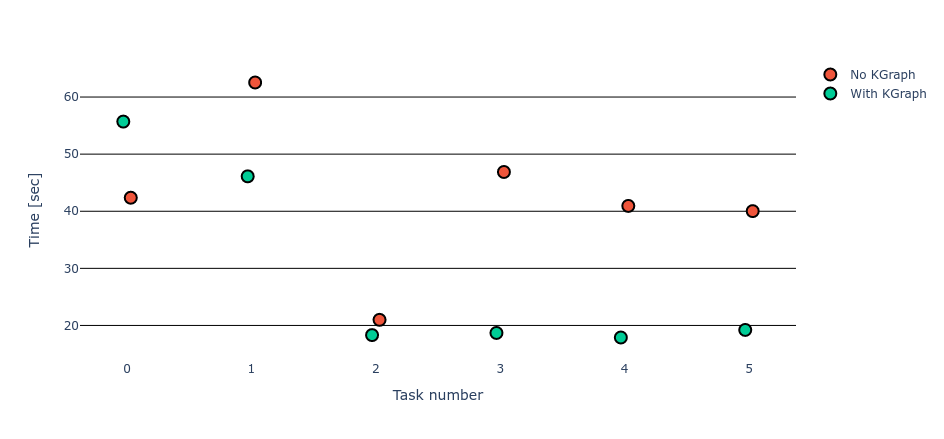
\includegraphics[width=\textwidth]{figures/results/random_push_time_vs}
    \caption{Comparing average total time to complete a task out of then runs for a pushing task. For the edge parameterizations once with the use of \ac{kgraph} action suggestions is leveraged indicated by \quotes{with \ac{kgraph}} and once with random selection indicted by \quotes{no \ac{kgraph}}.}%
    \label{fig:random_push_time_vs}
\end{figure}


\begin{table}[H]
    \centering
    \begin{tabular}%
      {
        >{\raggedright\arraybackslash}p{0.10\textwidth}
        >{\raggedright\arraybackslash}p{0.35\textwidth}
      |p{0.4cm}p{0.4cm}p{0.4cm}p{0.4cm}p{0.4cm}p{0.4cm}}
      \multicolumn{2}{c|}{Number of Tasks in experience} &0&1&2&3&4&5\\\toprule
      \multirow{4}{0.1\textwidth}{With \ac{kgraph} suggestions} 
      &Number of \textit{nonlinear-push-model-1} parameterizations&4&5&8&10&10&10\\
      &Number of \textit{nonlinear-push-model-2} parameterizations&5&4&2&0&0&0\\
      & \textit{nonlinear-push-model-1} selected in total push actions [\%]&44&56&80&100&100&100\\
      & \textit{nonlinear-push-model-2} selected in total push actions [\%]&56&44&20&0&0&0\\\midrule
      \multirow{4}{0.1\textwidth}{Without \ac{kgraph} suggestions} 
      &Number of \textit{nonlinear-push-model-1} parameterizations&4&3&7&5&4&5\\
      &Number of \textit{nonlinear-push-model-2} parameterizations&5&5&3&5&6&4\\
      & \textit{nonlinear-push-model-1} selected in total push actions [\%]&44&38&70&50&40&56\\
      & \textit{nonlinear-push-model-2} selected in total push actions [\%]&56&62&30&50&60&44\\
    \end{tabular}
    \caption{Influence of \ac{kgraph} suggestions in selecting the (\ac{MPPI}, \textit{nonlinear-push-model-1}) parameterization versus selecting the (\ac{MPPI}, \textit{nonlinear-push-model-2}) parameterization for push actions.}%
    \label{table:rand_push_model1_vs_model2}
\end{table}


The \ac{kgraph} favours the \ac{MPPI} controller with \textit{nonlinear-push-model-2} as can be seen in \Cref{table:rand_push_model1_vs_model2}. The nonlinear-push-model-2 parameterization does not only have a lower execution time compared to the nonlinear-push-model-1 parameterization, it also has a lower \ac{PE} as can be seen in \Cref{fig:random_push_pe_vs}.

\begin{figure}[H]
    \centering
    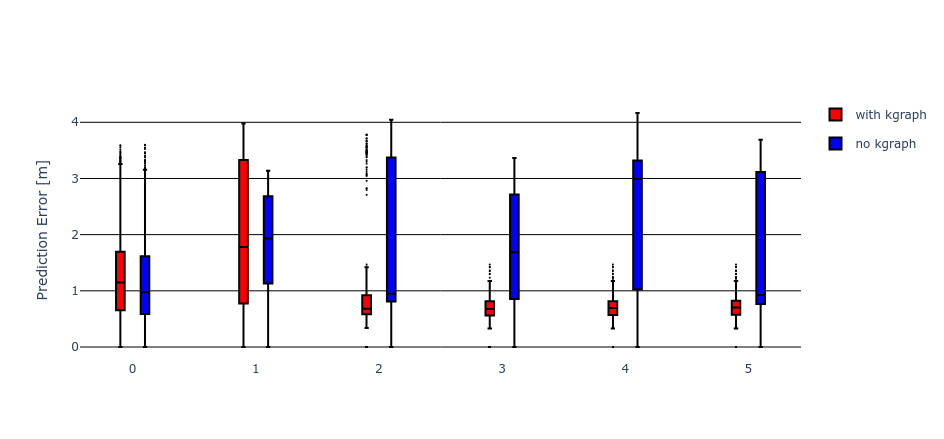
\includegraphics[width=\textwidth]{figures/results/random_push_pe_vs}
    \caption{Box plot of the \acl{pe}, a comparison between \ac{kgraph} action suggestions and randomly selection.}%
    \label{fig:random_push_pe_vs}
\end{figure}

The proposed framework has been compared against itself, now it is compared to the state-of-the-art in the upcoming section.\bs

\section{Comparison with State-of-the-Art}%
\label{sec:compare_with_related_papers}
In the introduction \Cref{table:sota_and_3_topics} was presented. That table presents state-of-the-art methods and the subset of the three main topics that they include (the three topics; learning system models, the \ac{NAMO} problem and nonprehesile pushing). Now that table is augmented with an extra column augmented to the table. This extra column indicates the testing methric that state-of-the-arts uses and underlines the metric that is compared between the proposed framework and the state-of-the-art.\bs

\noindent
\begin{table}[H]
  \centering
  \rowcolors{2}{white}{myEvenLighterColor}
  \begin{tabular}
    {>{\raggedright\arraybackslash}P{1.5cm}%
      >{\raggedright\arraybackslash}P{1.0cm}%
      >{\centering\arraybackslash}P{1.4cm}%
      |>{\centering\arraybackslash}P{1.4cm}%
      >{\centering\arraybackslash}P{1.4cm}%
      |>{\centering\arraybackslash}P{1.4cm}%
      >{\centering\arraybackslash}P{1.4cm}%
      |>{\raggedright\arraybackslash}P{3.0cm}
    }
    &&& \multicolumn{2}{c|}{\ac{NAMO}} & \multicolumn{2}{c}{\shortstack[c]{Specify object\\target poses}}\\
  Author&
  Citation&
  Learns\newline object\newline dynamics&
  \vspace{-0.2cm}\rotatebox{50}{prehesile}&
  \vspace{-0.4cm}\rotatebox{50}{nonprehesile}&
  \vspace{-0.2cm}\rotatebox{50}{prehesile}&
  \vspace{-0.4cm}\rotatebox{50}{nonprehesile}&
  method metric\\\toprule
  \citeauthor{ellis_navigation_2022} &          \cite{ellis_navigation_2022} &          \cmark& \xmark& \cmark& \xmark& \xmark& success rate\\
  \citeauthor{sabbaghnovin_model_2021} &        \cite{sabbaghnovin_model_2021} &        \cmark& \cmark& \xmark& \cmark& \xmark& success rate, execution time prediction error, final position error\\
  \citeauthor{scholz_navigation_2016} &         \cite{scholz_navigation_2016} &         \cmark& \cmark& \xmark& \xmark& \xmark& \underline{runtime}, \underline{planning time}, \underline{number of}\underline{replannings} number of calls to update model\\
  \citeauthor{vega-brown_asymptotically_2020} & \cite{vega-brown_asymptotically_2020} & \xmark& \cmark& \xmark& \cmark& \xmark& computation time\\
  \citeauthor{wang_affordancebased_2020} &      \cite{wang_affordancebased_2020} & \cmark& \xmark& \cmark& \xmark& \xmark& \underline{computation and} \underline{execution time}\\
  Groote & Proposed Framework & \xmark/\cmark& \xmark& \cmark& \xmark& \cmark&
\end{tabular}
\caption{Overview of recent state-of-the-art papers that include a subset of the 3 topics (learning system models, \ac{NAMO}, and nonprehensile pushing). The \textit{grasp-push} and \textit{grasp-pull} refer to prehensile push and pull manipulation, \textit{gripped} refers to fully gripping and lifting objects for manipulation, \textit{pushing} refers to nonprehensile push manipulation. The test metric indicates the testing method used by the paper, where the underlined metric is used to compare against the proposed framework.}%
\label{table:sota_vs_results_proposed method}
\end{table}

A comparison with two state-of-the-art papers is made, that is accomplished by recreating the environment that the state-of-the-art has used during testing. With \citeauthor{scholz_navigation_2016} the number of replannings are compared, with \citeauthor{wang_affordancebased_2020} the computation and execution time is compared.\bs




\paragraph{Comparing Success Rate with \citeauthor{ellis_navigation_2022}}
\todo{This can use some extra review here, it is unclear}
% \citeauthor{ellis_navigation_2022} claims to push with a success rate \todo{Corrado: perhaps eleborate on that 100 percent, how does ellis define that?} of a 100\%~\cite{ellis_navigation_2022}. The test environment that \citeauthor{ellis_navigation_2022} has used is very similar to the random pushing task discussed in \Cref{sec:randomisation}. For both the random driving task and the random pushing task the success rate is 100\%. Meaning that every driving or pushing subtask was successfully completed. It is even so that for the result of the random push task (displayed in \Cref{fig:rand_push_full_pred,fig:random_push_all_times,fig:random_push_with_without_kgraph}) the number of hypotheses is equal to the number of subtasks \todo{Corrado: How do I see this? unclear to tthe reader}. Meaning that every subtask is completed by the first hypothesis generated. Both similar experiments from \citeauthor{ellis_navigation_2022} and this thesis have a 100\% success rate for similar
% , allowing us to conclude that the results are comparable.



% \paragraph{Comparing something TODO with \citeauthor{sabbaghnovin_model_2021}}
% \citeauthor{sabbaghnovin_model_2021} grasp-pushes and grasp-pulls a walker object to two new target configurations~\cite{sabbaghnovin_model_2021}. The task is mimicked by pushing a box object of equal dimensions to the same target configurations. Compared to \citeauthor{sabbaghnovin_model_2021} average of 125 and 160 seconds to complete task 1 and task 2 the proposed framework takes an average of only 27 and 33 seconds respectively (10 seconds computation time) to complete similar tasks. The decrease in total time allows to conclude that the proposed frameworks improve upon the method proposed by~\citeauthor{sabbaghnovin_model_2021}.\bs \todo{Corrado: So your pushing controllers are performin better than prehensile manipulation? amazing, but doub}



% \paragraph{Comparing something TODO with \citeauthor{vega-brown_asymptotically_2020}}
% \citeauthor{vega-brown_asymptotically_2020} has a task that pushes two boxes into a goal region. It takes around 300 seconds to return a hypothesis~\cite{vega-brown_asymptotically_2020}. \todo{Corrado: What do you mean? for the next sentce}Both pushing tasks can be compared with two separate pushing tasks from the random push environment. By doubling the time to push a single object to its target configuration, $2 \cdot 30 = 60$ seconds both tasks could be compared. However, the point of \citeauthor{vega-brown_asymptotically_2020} paper is that a global minimal task is sought. The proposed framework randomly selects a subtask and tries to complete it to then move to the next randomly selected subtask. A global minimum is thus not sought and both papers can therefore not be compared properly.\todo{Corrado: Then why including it in the comparison?}\bs



% \paragraph{Comparing Computation and Execution Time }
% Three state-of-the-art papers that use computation and execution time as the testing metrics are compared to the proposed framework. To accomplish a fair comparison the environments that have been used in the \todo{Corrado: Where do I see this?} citations are rebuilt in the pybullet software. The results are then directly compared to conclude that the proposed framework is as good as or even better in terms of computation time and execution time for similar tasks.\bs


\paragraph{Comparing Computation and Execution time with \citeauthor{wang_affordancebased_2020}}
\citeauthor{wang_affordancebased_2020} combines the \ac{NAMO} problem with learning object dynamcs. Their papar tests their method with a task to drive toward a target pose, where a chair is blocking the path~\cite{wang_affordancebased_2020}. The environment is mimicked with three walls and a red box on the spot where is chair stands. The origal and mimicked robot environments can be seen in \Cref{fig:wang}.\bs 

\begin{figure}[H]
    \centering
    \begin{subfigure}{.49\textwidth}
    \centering
    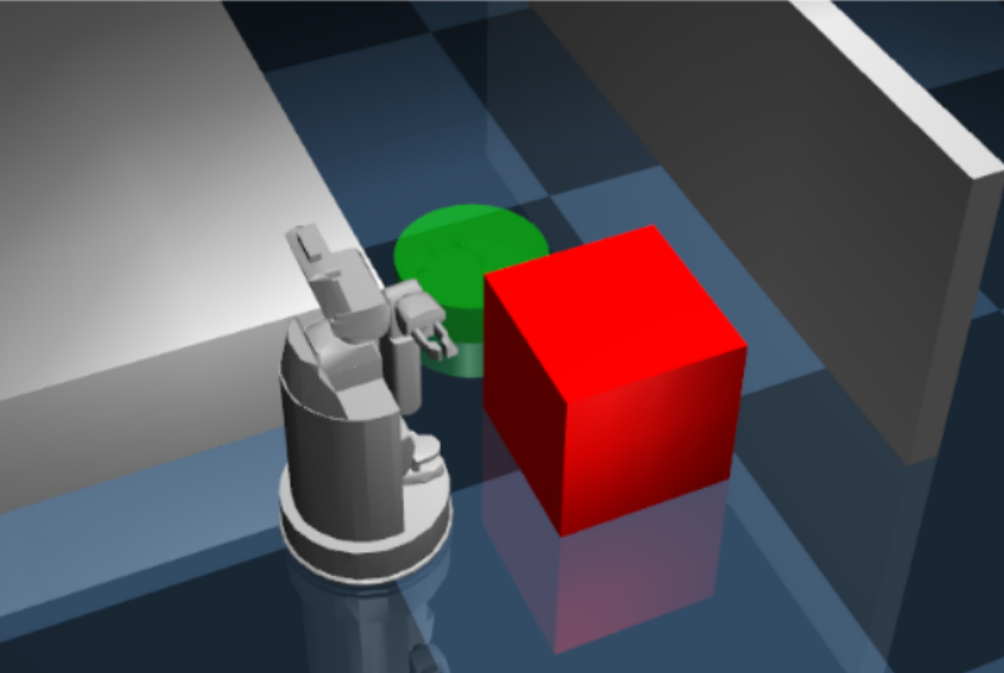
\includegraphics[width=0.9\textwidth]{figures/results/wang_env}
    \caption{\citeauthor{wang_affordancebased_2020} simulation environment.}%
    \label{subfig:wang_env}
    \end{subfigure}
    \hfill
    \begin{subfigure}{.49\textwidth}
    \centering
    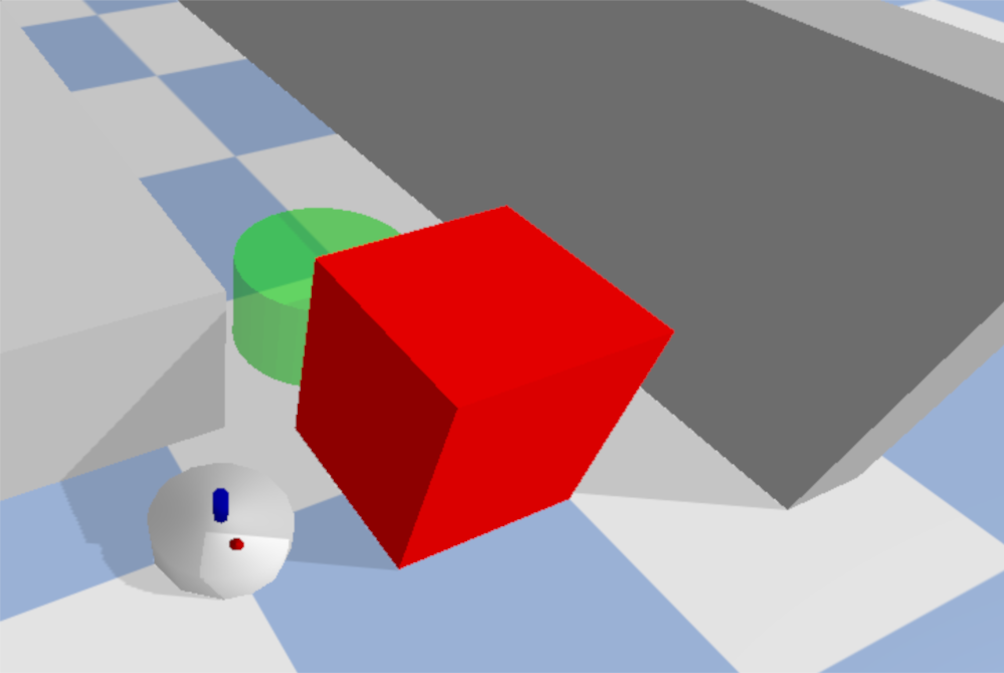
\includegraphics[width=0.9\textwidth]{figures/results/wang_mimick}
    \caption{Recreated simulation environment.}%
    \label{subfig:wang_mimick}
    \end{subfigure}
    \caption{Two similar environments and tasks, the robots are taskedto drive toward a target position indicated with the green ghost poses. In both environment a direct path is blocked by the red box.}%
    \label{fig:wang}
\end{figure}


\citeauthor{wang_affordancebased_2020} solves the task three times, the average search-, execute- and total time over these three executions is displayed in \Cref{table:wang_vs_mimick}. Note that \citeauthor{wang_affordancebased_2020} splits the search time in two categories (time to estimate affordance of an object and time to optimize the trajectory. The recreated or mimicked environmnet displayed in \Cref{subfig:wang_mimick} is solved ten times, every time starting without environmental knowledge and thus an emtpy \ac{kgraph}. The avarage search, execute- and total time over these then executions is also displayed in \Cref{table:wang_vs_mimick}.\bs

\begin{table}[H]
    \centering
    \begin{tabular}%
    {>{\raggedright\arraybackslash}p{0.2\textwidth}|%
    >{\centering\arraybackslash}p{2cm}%
    >{\centering\arraybackslash}p{2cm}}%
    Author &\citeauthor{wang_affordancebased_2020} & Groote \\\toprule
    search time [sec]  & 109 & 26 \\
    execution time [sec]  & 67 & 4 \\
    total time [sec] & 176 & 30
    \end{tabular}
    \caption{Average execute-, search and total times for a repeated task solved three times. The task involves learning object dynamcis and the \ac{NAMO} problem and can be visualise in \Cref{fig:wang}.}%
    \label{table:wang_vs_mimick}
\end{table}


In this experiment we compare against Wang. The goal is to reach a target location,but the robotis reuiredto free the path first. The visialized in fig.

\todo{Some conclusion on the table above}


% \paragraph{Comparing Prediction Error}
% \citeauthor{sabbaghnovin_model_2021} displays the final position errors for a selection of objects which range from 0.05 to 0.6 meters. A success threshold is set to 0.1 meters, which determines that the object is at its target location~\cite{sabbaghnovin_model_2021}. The success threshold in this thesis is set to a staggering 0.9 meters,\todo{Corrado: But then how can you compare success rate if you have different metrics for success?} thus it is concluded an object has reached its target position, whilst it is still 0.9 meters from its target configurations. This thesis does not try to reach optimal control, it tries to select the best controller in the available set of controllers. If the same controller from \citeauthor{sabbaghnovin_model_2021} would be available, then similar final position errors would be obtained. It can be concluded that the prediction error \todo{Corrado: Not position errro?}of the proposed framework is worse compared to this state-of-the-art. The reason is that the proposed framework focuses on improving the control selection and action sequences over time, and not on lowering final prediction errors.\bs

\paragraph{Comparing Number of Replanning times}
\todo[inline]{\cite{scholz_navigation_2016}}
\todo{recreate this envionrment, run 10 tests and compare the search and execution time, as well at the number of call toward the planner}
\todo{additinoally execute this environment a twice in a row, show that the execution number of call to the planner drops, theand the execution time drops}


